\documentclass[twoside,11pt]{article}

\usepackage{blindtext}

% Any additional packages needed should be included after jmlr2e.
% Note that jmlr2e.sty includes epsfig, amssymb, natbib and graphicx,
% and defines many common macros, such as 'proof' and 'example'.
%
% It also sets the bibliographystyle to plainnat; for more information on
% natbib citation styles, see the natbib documentation, a copy of which
% is archived at http://www.jmlr.org/format/natbib.pdf

% Available options for package jmlr2e are:
%
%   - abbrvbib : use abbrvnat for the bibliography style
%   - nohyperref : do not load the hyperref package
%   - preprint : remove JMLR specific information from the template,
%         useful for example for posting to preprint servers.
%
% Example of using the package with custom options:
%
% \usepackage[abbrvbib, preprint]{jmlr2e}

\usepackage{jmlr2e}
\usepackage{algorithm}
\usepackage{algpseudocode}

% Definitions of handy macros can go here

\newcommand{\dataset}{{\cal D}}
\newcommand{\fracpartial}[2]{\frac{\partial #1}{\partial  #2}}

% Heading arguments are {volume}{year}{pages}{date submitted}{date published}{paper id}{author-full-names}

\usepackage{lastpage}
\jmlrheading{23}{2023}{1-\pageref{LastPage}}{}{}{}{}

% Short headings should be running head and authors last names

\ShortHeadings{Optimal allocation design for EV chargers in Madison}{Optimal allocation design for EV chargers in Madison}
\firstpageno{1}

\begin{document}

\title{Optimal allocation design for EV chargers in Madison}

\author{\name Zhengwei Tong \email ztong33@wisc.edu \\
       \addr Department of Mathematics\\
       University of Wisconsin-Madison\\
       Madison, WI 53706, USA
       \AND
       \name Michael C. Ferris \email ferris@cs.wisc.edu \\
       \addr Department of Computer Science\\
       University of Wisconsin-Madison\\
       Madison, WI 53706, USA}

% \editor{}

\maketitle

\begin{abstract}%   <- trailing '%' for backward compatibility of .sty file
The increasing popularity of electric vehicles (EVs) has led to a growing demand for convenient and reliable charging infrastructure. As cities around the world work to promote sustainable transportation, an important question that arises is how to optimally allocate EV chargers to meet the needs of EV drivers while also considering factors such as cost, social event impact, and spatial distribution. In this study, we focus on the city of Madison, Wisconsin and investigate the optimal allocation of EV chargers in the city. We aim to identify the most efficient and customer-satisfied allocations for EV chargers, taking into account factors such as charging price, distance to final destination and driver's own preferences. We built a simualtion model testing the design of two parking lots and limited number of chargers under different scenarios, and the optimal result shows a concentration behavior of the chargers. The research result will provide valuable insights on pricing strategy for policymakers and city planners as they work to promote the adoption of EVs and support the transition to a more sustainable transportation system.

\end{abstract}

% \begin{keywords}
%   keyword one, keyword two, keyword three
% \end{keywords}

\section{Introduction}


\subsection{Background}
Electric Vehicles (EVs) have become increasingly popular in recent years, as they offer numerous environmental and economic benefits. With the growing adoption of EVs, the demand for efficient and accessible charging infrastructure has risen significantly. An important aspect of developing this infrastructure is determining the optimal allocation of EV chargers to maximize utility for users. Factors such as traffic flows and pricing strategies play a crucial role in the decision-making process for allocating charging stations.

The objective of this paper is to investigate the impact of different traffic flows and pricing strategies on the optimal allocation of EV chargers. Specifically, we focus on two distinct traffic flow scenarios: normal days and game days. By analyzing the effects of these scenarios on charger allocation, we aim to provide valuable insights that can inform policymakers, EV charging infrastructure providers, and other stakeholders in their decision-making process.

To achieve our objectives, we will employ a simulation model that takes into account various factors, including traffic flows, pricing strategies, and charger availability. The model will use a utility function to evaluate different allocation plans, ultimately identifying the best allocation strategy under each scenario.

Through this research, we hope to contribute to the existing body of knowledge on EV charger allocation and offer practical recommendations for optimizing charging infrastructure. By considering the influence of traffic flows and pricing strategies on charger allocation, we aim to promote the efficient and sustainable growth of the EV market, ultimately benefiting both users and the environment.

\subsection{Literature Review}

In this section, we will review the existing literature on EV charger allocation, traffic flows, and pricing strategies to provide context for our study and identify areas where our research can make a valuable contribution.

EV charger allocation: Numerous studies have explored various aspects of EV charger allocation, such as placement strategies, charger types, and the role of geographical factors. These studies have helped to establish a foundation for understanding the complexities of allocating EV chargers in a way that maximizes utility for users.

\textbf{Details to be added.}
% Study 1 (arXiv link) - Discuss the main findings of this study related to charger allocation.
% Study 2 (arXiv link) - Explain the contributions of this study to the field of EV charger allocation.
% Traffic flows: The impact of traffic flows on EV charger allocation has been an important area of investigation. Researchers have examined how different traffic patterns, such as daily fluctuations, seasonal variations, and special events, can influence the demand for EV charging and the optimal allocation of charging stations.

% Study 3 (arXiv link) - Summarize the main findings of this study related to traffic flow impacts on EV charger allocation.
% Study 4 (arXiv link) - Describe the insights provided by this study on the relationship between traffic flows and EV charger allocation.

% Pricing strategies: Pricing strategies play a significant role in determining the usage patterns of EV charging stations and, consequently, the optimal allocation of chargers. Several studies have focused on the effects of different pricing strategies, such as time-of-use pricing, dynamic pricing, and flat rate pricing, on the demand for EV charging and charger allocation decisions.

% - *Study 5* (arXiv link) - Discuss the main findings of this study related to the impact of pricing strategies on EV charger allocation.
% - *Study 6* (arXiv link) - Explain the contributions of this study to the understanding of pricing strategies and their effects on charger allocation.

% In summary, the existing literature has provided valuable insights into various aspects of EV charger allocation, including the influence of traffic flows and pricing strategies. However, there remain gaps in the literature, particularly in terms of the combined effects of these factors on charger allocation under specific scenarios such as normal days and game days. Our study aims to address these gaps by conducting a detailed simulation-based analysis of the impact of different traffic flows and pricing strategies on the optimal allocation of EV chargers.


% Electric vehicle (EV) charging infrastructure is a rapidly evolving field, with various researchers and organizations working to improve the technology and make it more widely available. Current EV chargers can be broadly categorized into three types: Level 1, Level 2, and DC fast charging. Level 1 chargers are the most basic and slowest, typically using a standard 120-volt household outlet to charge the EV. Level 2 chargers use a 240-volt outlet, similar to that used for an electric dryer or range, and can charge an EV much more quickly. DC fast chargers, also known as Level 3 chargers, use direct current (DC) power to charge an EV in a matter of minutes rather than hours.

% Researchers have made significant contributions to the development of EV charging infrastructure, including the development of more efficient and cost-effective charging equipment, the expansion of charging networks, and the integration of renewable energy sources into the charging process. For example, a team from the University of California, Davis developed a model to optimize the placement of EV charging stations, taking into account factors such as the number of potential users, the availability of renewable energy sources, and the cost of the charging equipment. Another research group at the Technical University of Denmark developed a system that uses solar panels and energy storage to power EV charging stations, reducing the environmental impact of the charging process.

% In addition to the development of EV charging equipment, researchers have also focused on the problem of EV charger distribution or allocation design. This involves determining the optimal locations for EV charging stations, taking into account factors such as the number and distribution of potential EV users, the availability of renewable energy sources, and the cost of the charging equipment.

% One of the main challenges in this area is to ensure that charging infrastructure is accessible to as many EV users as possible, while also minimizing the costs associated with building and maintaining the charging stations. Researchers have used various methods to address this challenge, including mathematical modeling, network optimization, and machine learning techniques.

% For example, a team from the Technical University of Munich used a mathematical model to optimize the placement of EV charging stations in urban areas, taking into account factors such as the distribution of EV users and the availability of renewable energy sources. Another research group at the University of California, Berkeley used a network optimization approach to determine the optimal locations for EV charging stations on a regional scale, considering the potential demand from EV users and the cost of building and operating the charging stations.

% Additionally, researchers have employed machine learning techniques to predict the demand for EV charging stations and optimize their distribution. For instance, a team from the University of California, San Diego used a machine learning algorithm to predict the demand for EV charging stations in a given region and determine the optimal locations for the charging stations based on the predicted demand.

% However, with respect to the specific parking and charging details, previous researches have not simulated the details. In this paper, we expect to use Madison city as an example to do detailed simulation of the charging behavior, and would like to see how these behaviors going to change the final optimal allocation design.

\section{Model}
\subsection{Background}


The city of Madison presents a significant opportunity for the implementation of electric vehicle (EV) charging infrastructure. There are a plethora of available parking lots in the city, each of which has the potential to serve a specific region and meet the demands of local parking needs. In particular, the downtown and campus areas of Madison exhibit a higher density of parking lots, reflective of the increased demand for parking in these areas. In light of this, it is assumed that all EV charging stations will be situated within existing parking lots, as EVs typically utilize their parking time for charging. Furthermore, indoor parking lots provide an optimal environment for EV charging, as their construction design can facilitate the maintenance of desirable temperature and voltage levels, which are crucial for effective battery charging.

To simplify the model, the city of Madison has been divided into sixteen equally-sized areas, with two parking lots assumed to cover each area. This model can be easily adapted to account for additional parking lots and different area divisions, providing a flexible framework for the implementation of EV charging infrastructure in Madison.
\begin{figure}[t]
    \includegraphics[width = 0.8\textwidth]{figure/madison.png}
    \centering
    \caption{The city division and parking lots assumption}
    \label{fig:madison}
    \end{figure}



\subsection{Model Overview}
In order to accurately simulate the scenario of EV charging infrastructure implementation in Madison, a comprehensive model was developed that is divided into three key components: Data Generation, Drivers' Choice, and Parking Simulation. The flowchart~\ref{fig:flowchart} provided illustrates the structure of the model and the inter-dependencies between the various components.

Given the paucity of available data, the Data Generation component of the model is crucial in generating synthetic data to be used in the subsequent stages of the model. As such, the validity of the results obtained is contingent upon the quality of the data generated. However, when real-world data becomes available, it can be easily integrated into the model by modifying the Data Generation component, thereby enabling the generation of results that are reflective of reality.

\begin{figure}[t]
    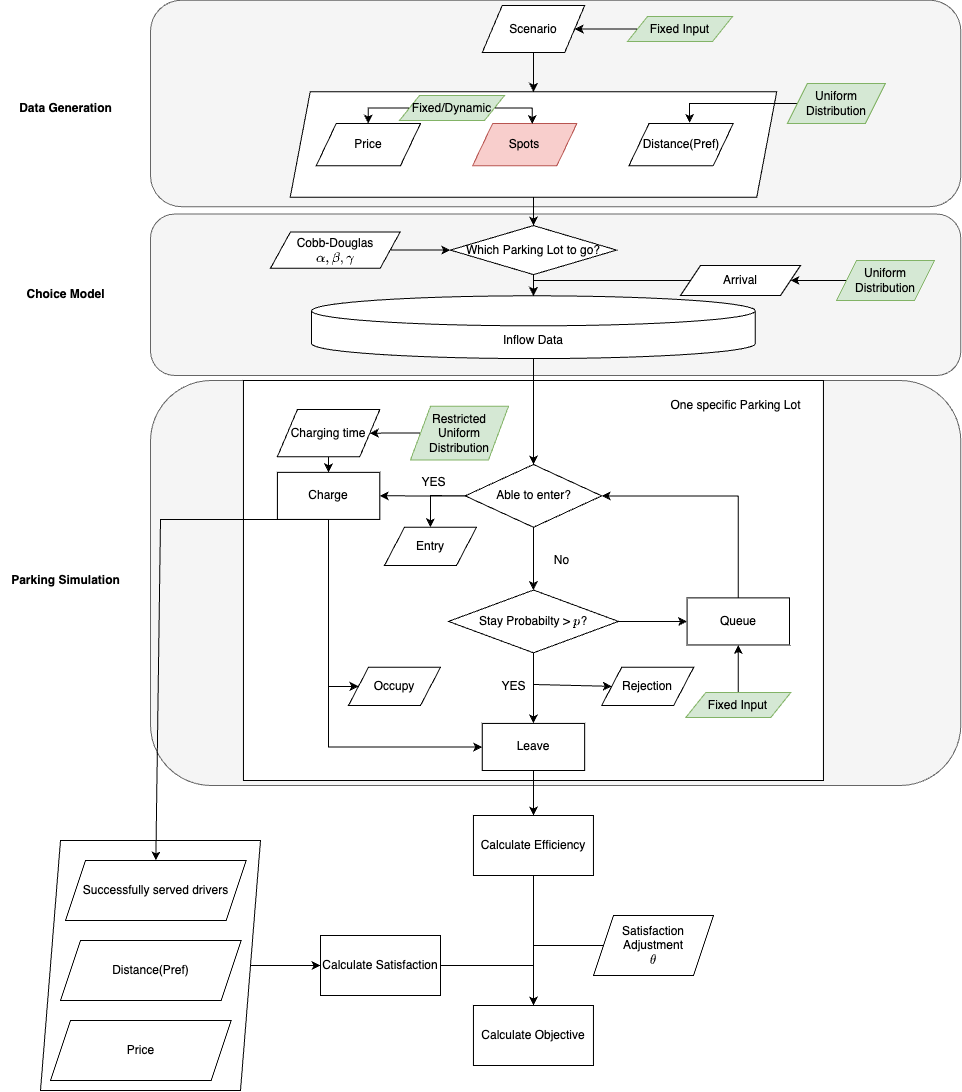
\includegraphics[width = 0.8\textwidth] {figure/flowchart.png}
    \centering
    \caption{The overall structure of the model}
    \label{fig:flowchart}
    \end{figure}



\subsection{Model Details}
\subsubsection{Data Generation}
\textbf{Scenario}: In our model, we consider parking and charging event happening in different scenarios: normal days and Game days. During normal days, we assume that the traffic flow is even over all regions. During Game days, because the high demand of parking near the stadium, there will be a certain period of time in a day that one parking lots will have heavy traffic. 

For simplicity, we set up a uniform distribution of incoming traffic flow on normal days. Namely, the drivers will arrive at the parking lot with equivalent time gap. While for Game days situation, we let 80\% of traffic flow arrives during 10\% of the time in a day to simulate the situation. 

\textbf{Price}: In our model, we assumed price is the one of the key factor influencing the driver's decision of which parking lot to go. The price can be a fixed number, or be selected dynamically within a certain range. For Game days scenario, we applied a \textbf{Gameday multiple} to modify the price to see the influence. 

\textbf{Spots}: Spots refer to the available chargers in certain parking lots, and we also considered this as one of the factors that will influence the driver's decision. We assumed under the budget, there will only be limited number of available chargers altogether to be implemented in the city. In most of our experiments, this number is set to be 20. 

\textbf{Distance(Pref)}: Distance refers to the distance from the parking lot to the driver's desired destination. Usually, people intends to park as close as possible to their destination, so this factor can also be understood as the preference value of the parking lots by each driver. The smaller the distance, the more preferable the parking lot. In our experiment, we generate this value from uniform distribution in certain range. 

\subsubsection{Choice Model}

The driver's choice can be viewed as a decision over utility of each parking lots. We intrdouced the well-know Cobb-Douglas utility function to simulate the decision process of each driver. With the input of price, spots, and distance, each driver will have an utility value of each parking lots. Based on the corresponding utility value, the driver will make a probability-based choice: The higher the value, the more possible the driver will choose certain parking lot. The reason we introduce the probability choice model is to simulate the possible unexpected decisions from drivers. 

More precisely, we have
utility function designed as
$$
\mu_{d_i}(l) = P^{\alpha} S^{\beta} D^{\gamma}
$$

where $d_i$ represents the $i$ th driver, $l$ represents the selected parking lot, $P$ represents Price, $S$ represents Spots, $D$ represents Distance. $\alpha, \beta, \gamma$ are parameters tuned for simulation. 

The decision function is 
$$
\mathbb{P}_{d_i}(l) = Bin(1, \mu_{d_i}(l))
$$

Based on the current position of each driver and decision made from the model, we can generate the incoming flow to each parking lots, which gives us the Inflow Data. 


\subsubsection{Parking Simulation}
The parking simulation can be divided into several small process: entering process, charging process, and queue process.

\paragraph{Entering Process}
When the driver arrives a certain parking lot, he/she may find two different situations: the parking lot does have available spot right now, or the parking lot is full and there's a queue for waiting. 

If there is an available spot, the driver will enter the lot and continue to charging process. If not, he/she has to join the queue. 

\paragraph{Charging Process}
After successfully entering the parking lot, the driver will start the charging process right away. We neglect the time gap for finding a specific spot, as this is not the main concern of the model. 

The charging time will depend on the current battery level of the car, therefore it varies from driver to driver. To simulate this situation, we applied a uniform distribution on determining the charging time. 

\paragraph{Queue Process}
If the driver didn't enter the parking lot and join the queue, then he/she must take the following procedure. 

The driver is supposed to stay at least for one time unit, and his/her patience is measured by the \emph{stay probability}. After each time unit, the driver's stay probability will decrease center amount, and once the stay probability goes under the threshold, the driver will leave the queue system and is designed to not come back. 

For each time unit, the driver will try to enter the parking lot. Because after each time unit, there will be some drivers finish charging, therefore there will be available spots open for the next driver. The entering rule follows first come, first serve, which means those who entered the queue system earlier and didn't leave will have priority to enter the system. 

Say the threshold is $p$, the decreasing amount is $\delta_p$, then the algorithm will be 

\begin{algorithm}
\caption{Driver Queue}
\label{alg:entry}
\begin{algorithmic}[1]
\If{$P_{stay} > p$}
\If{$Spot > 0$}
\State Enter System
\State Queue \textbackslash Driver
\Else
\State $P_{stay} \gets P_{stay} - \delta_p$
\EndIf
\EndIf
\end{algorithmic}
\end{algorithm}

\subsection{Evaluation Model}
Our evaluation model considers both the driver side and the designer side. For the driver, the rate of successful service, demand-meet of preference, and the price of charging are the primary considerations. For the designer, the occupancy rate of the chargers is the primary consideration. We use a satisfaction adjustment coefficient $\theta$ to balance the emphasis between the driver side and the designer side. The efficiency rate of chargers can also affect the balance between the two sides.

If the efficiency rate of chargers is above a certain threshold, such as 75\%, we prioritize driver satisfaction. By balancing the preferences of drivers and designers, our model can provide valuable insights for the development of EV charging infrastructure.

\section{Traffic Scenario}
In this section, we discuss and observe the behavior in two different traffic scenarios. The first scenario is the normal day situation, where the traffic flow is more uniform over all parking lots. The second scenario is the Game day situation, where the traffic flow is more concentrated in one parking lot.

\subsection{Normal Day Traffic}

If we turn off all the systems (like queue system, charging system)

\begin{figure}
    \centering
    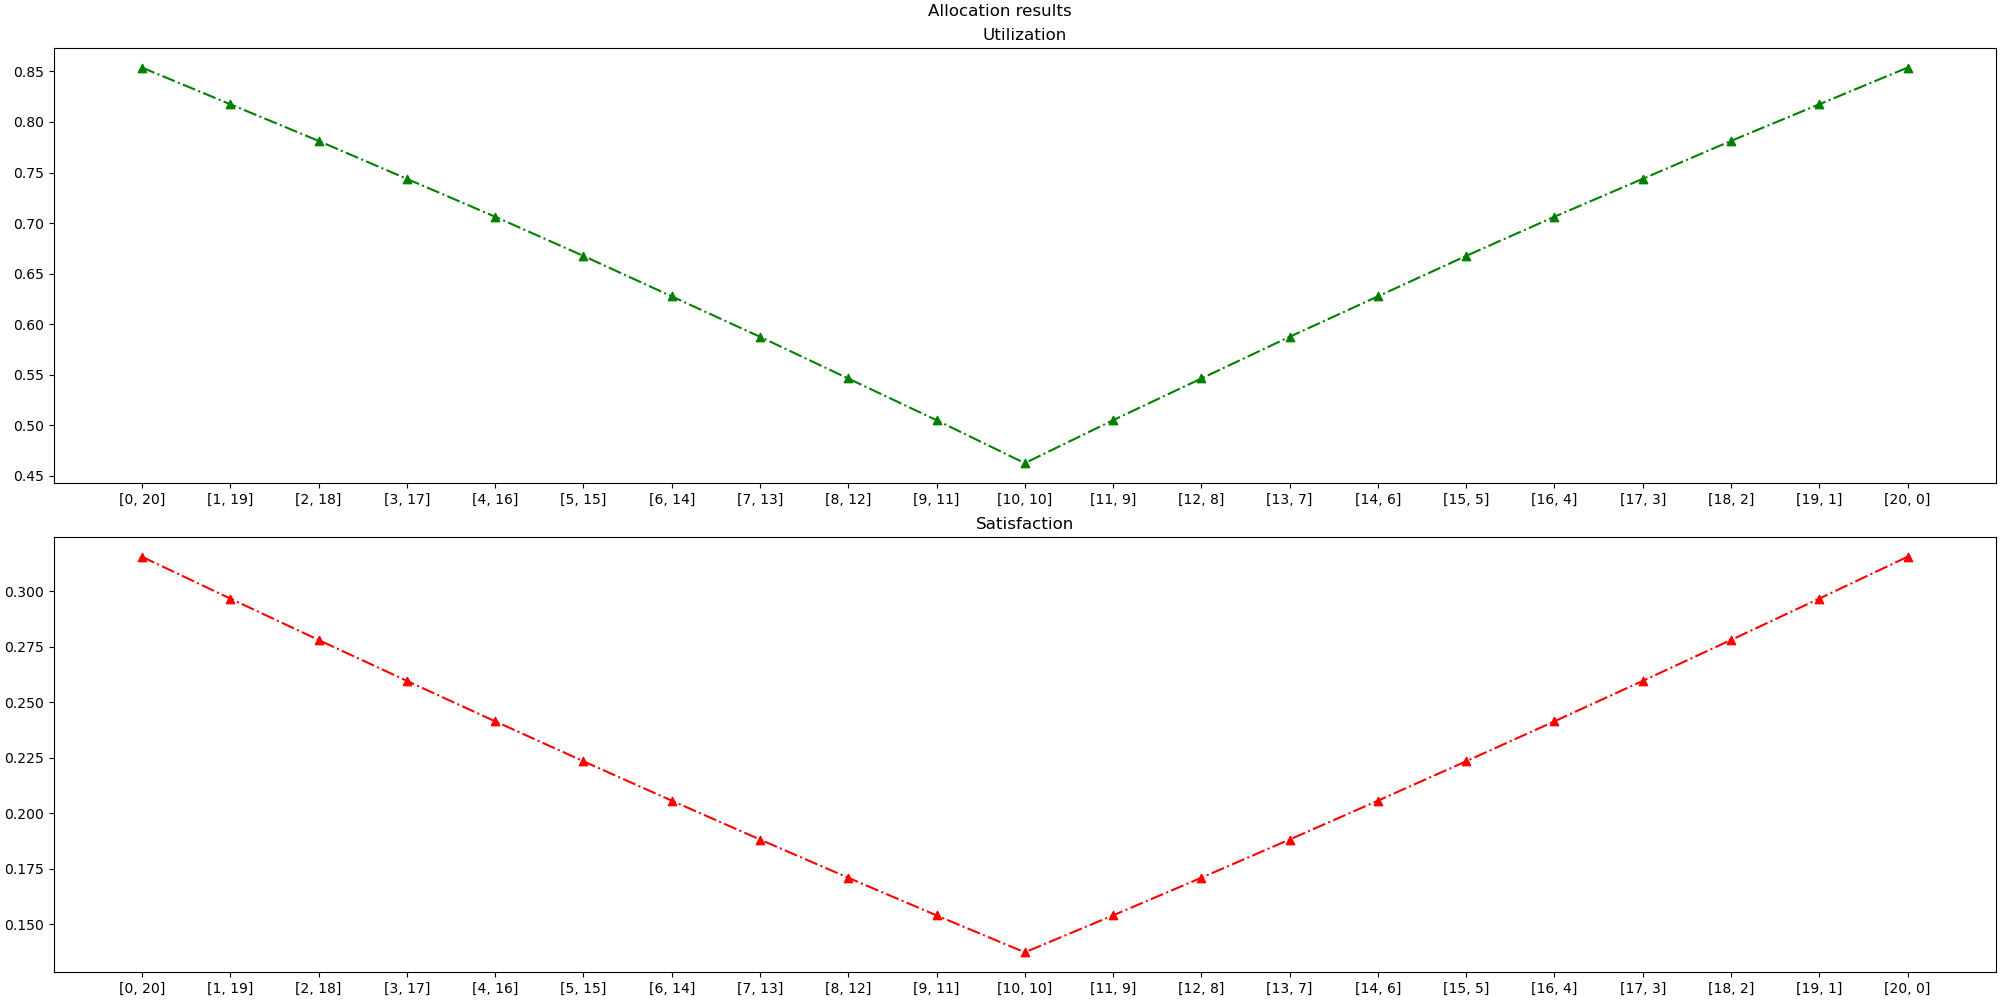
\includegraphics[width=\textwidth]{figure/traffic_scenario/all_clean.png}
\end{figure}


\section{Price Scenario}
In this section, we mainly discuss about the influence of the pricing strategy. We first discuss the situation under normal days, then discuss about the change of Game days, and how the pricing strategy can be adjusted to fit the situation. Our setup for this section is an even distribution of the chargers over all parking lots.

\subsection{Normal Day Situation}
If the price is controled to be equivalent, assume all other systems are turned off, then the driver only makes choice between two parking lots based on the distance. If all other criteria are the same, then they will make a random choice. 

\begin{figure}
    \centering
    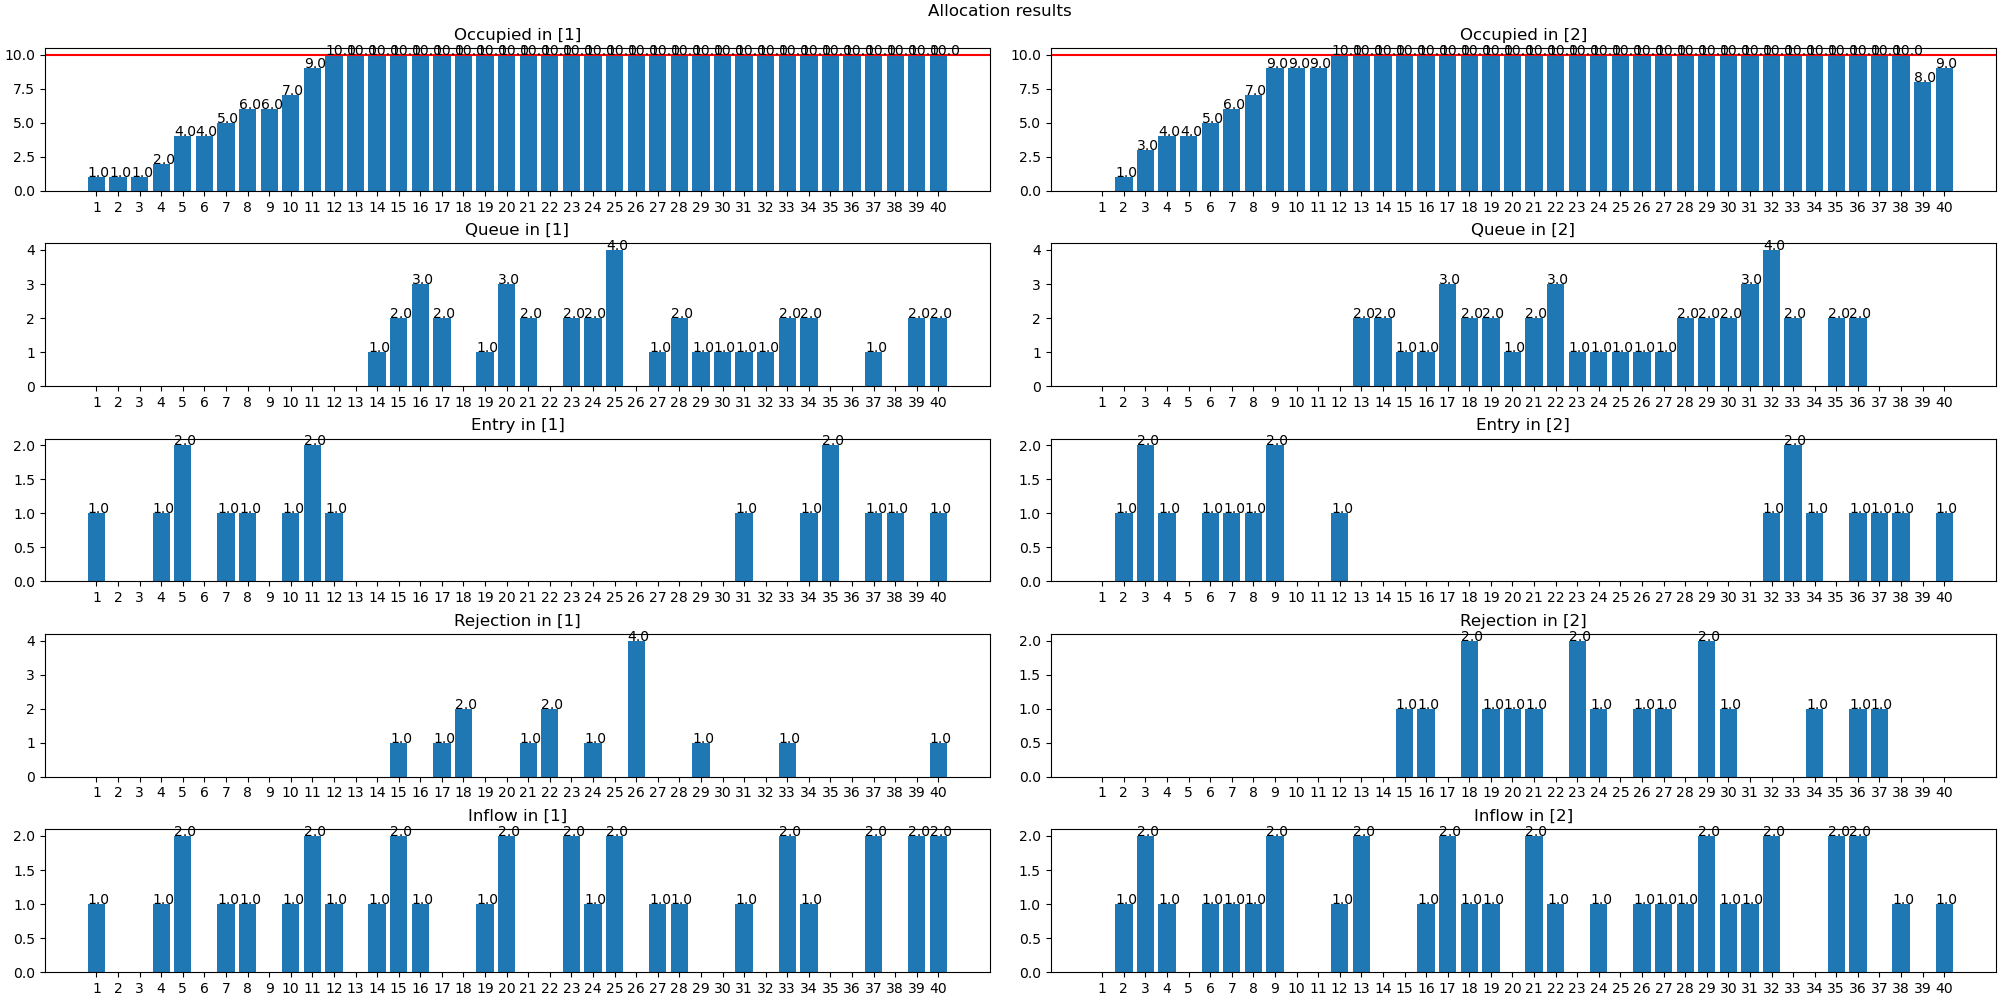
\includegraphics[width=\textwidth]{figure/price_scenario/all_clean.png}
\end{figure}


\section{Application}
\input{section/application.tex}


% Acknowledgements and Disclosure of Funding should go at the end, before appendices and references

% \acks{test}

% Manual newpage inserted to improve layout of sample file - not
% needed in general before appendices/bibliography.

\newpage

\appendix
\section*{Appendix A.}
\label{app:theorem}



\vskip 0.2in
\bibliography{paper}

\end{document}
